% Figure 7 of "The architecture of blockchain value: capabilities, pillars, and growth dynamics"
% (Papadogiannis, 2026, Front. Blockchain 9:1747512). Drawing code as in the author's manuscript.
% Compile with: pdflatex fig7_incentive_layering.tex
\documentclass[border=6pt]{standalone}
\usepackage{amsmath, amssymb}
\usepackage{tikz}
\usetikzlibrary{positioning, shapes, arrows.meta, calc, backgrounds}
\begin{document}
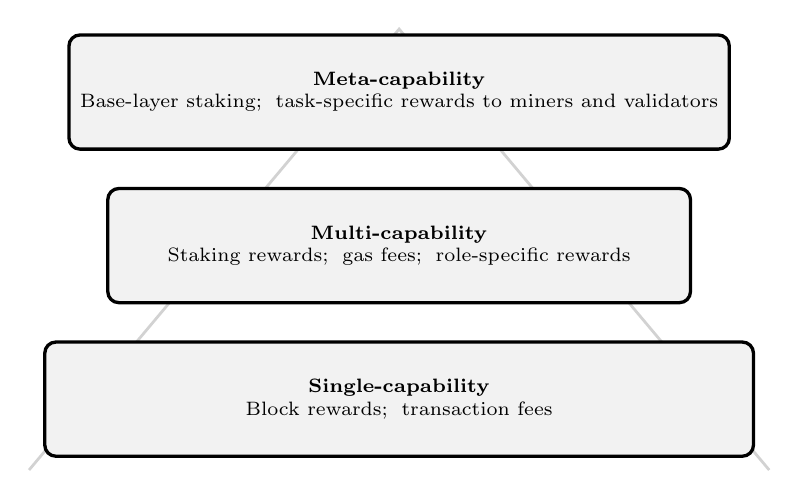
\begin{tikzpicture}[
  font=\scriptsize,
  layer/.style={draw=black, rounded corners=4pt, very thick, fill=gray!10, align=center, inner sep=4pt},
  ghost/.style={draw=gray!35, line width=1pt}
]

% Pyramid silhouette
\draw[ghost] (-4.7,-0.9) -- (0,4.7) -- (4.7,-0.9);

% Layers (centered, decreasing widths)
\node[layer, minimum width=9.0cm, minimum height=1.45cm] (single) at (0,0) {%
\textbf{Single-capability}\\
Block rewards;\; transaction fees
};

\node[layer, minimum width=7.4cm, minimum height=1.45cm] (multi) at (0,1.95) {%
\textbf{Multi-capability}\\
Staking rewards;\; gas fees;\; role-specific rewards
};

\node[layer, minimum width=5.8cm, minimum height=1.45cm] (meta) at (0,3.9) {%
\textbf{Meta-capability}\\
Base-layer staking;\; task-specific rewards to miners and validators
};

\end{tikzpicture}
\end{document}
